% DC_DC_converter.tex
%===============================Podkapitola: DC/DC měniče bez transformátoru========================
  \section{DC/DC měniče bez transformátoru}\label{ENZ:kap_DC_DC}
    \subsection{Vymezení pojmů a základních požadavků}
      DC - DC měniče jsou obvody sloužící k regulaci elektrické energie, které mění vstupní
      stejnosměrně napětí U1 na jiné výstupní stejnosměrné napětí U2. Budeme se přitom zabývat
      měniči tzv. \emph{napěťového typu}, což jsou měniče napájené konstantním vstupním napětím z
      napěťového zdroje, nikoliv proudem, z proudového zdroje. V této kapitole se omezíme pouze na
      měniče bez transformátoru, které tedy neumožňuji galvanické oddělení výstupu od vstupu
      \cite{Patocka}.

      Každý měnič sestává z vlastního silového obvodu a řídicí elektroniky (regulačních obvodů).
      Silové obvody nesmí využívat při regulaci energie rezistorů a proto se mohou skládat jen ze
      \textbf{spínačů} a \textbf{akumulačních prvků}, tj. \emph{indukčnosti} a \emph{kapacit}.

      \subsubsection{Napájecí zdroj a zátěž měniče}
        \begin{figure}[b]
          \centering
          \subfloat[náhradní schéma akumulátoru]{\label{enz:fig_nahr_sch_aku}
            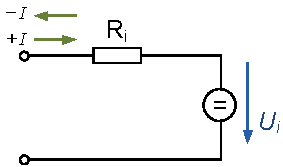
\includegraphics[width=0.4\linewidth]{patocka_aktivni_zatez_nahrad_sch.pdf}}
           \hfill 
           \subfloat[náhradní schéma stejnosměrného elektromotoru s cizím
                     buzením]{\label{enz:fig_nahr_sch_ss_motor}
            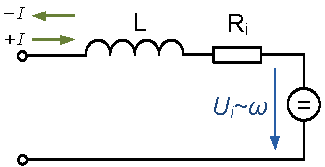
\includegraphics[width=0.4\linewidth]{patocka_aktivni_zatez_ss_mot_nahrad_sch.pdf}}
          \caption{Aktivní zátěž.}
          \label{enz:fig_aktivni_zatez}
        \end{figure}
        DC/DC měniče mohou přenášet energii z principu oběma směry. Mohou tedy čerpat energii ze
        zdroje a dodávat ji do zátěže nebo také opačně energii čerpat ze zátěže a dodávat ji do
        zdroje. Pojmy zátěž a zdroj je proto nutné chápat v širším slova smyslu.
        \begin{itemize}
          \item Zdrojem s konstantním napětím $U_1$, schopným dodávat i akumulovat energii, je
                akumulátor. Použijeme-li jako zdroj např. usměrňovač se sběrným kondenzátorem, pak
                není schopen dlouhodobě jímat energii z měniče, tj. dlouhodobě nesmí ve střední
                hodnotě převládat směr proudu do kladné svorky zdroje (krátkodobě, v okamžité
                hodnotě, je takový směr možný). Nabíjením sběrného kondenzátoru by totiž rostlo
                napětí $U_1$. Tomu lze zabránit přeměnou dodávané energie na teplo ve vybíjecím
                rezistoru, či na Zenerově diodě, zapojené paralelně ke sběrnému kondenzátoru.
          \item Z hlediska schopnosti spotřeby či dodávky energie, lze rozlišovat zátěž
                \emph{aktivní} a \emph{pasivní}. Aktivní zátěži je opět např. akumulátor, ale třeba
                i stejnosměrný motor. Jeho náhradní zapojeni, platné v ustáleném stavu, je uvedeno
                na obr. 1 1). Vnitřní rotační (pohybové) indukované napětí je úměrně otáčkám, proud
                pak momentu na hřídeli a to včetně znamének.
        \end{itemize}

        Teče-li proud ve  střední hodnotě do zátěže (+I), pak motor pohání, tj. mění elektrickou
        energii na mechanickou (pracuje v \emph{motorickém režimu}). Teče-li ze zátěže (-I), pak
        motor brzdí, tj. mění z vnějšku dodávanou mechanickou energii na energii elektrickou
       (pracuje v \emph{generátorickém režimu}).
       
      \subsubsection{Pracovní kvadranty}
         \begin{figure}[ht!]
           \centering
           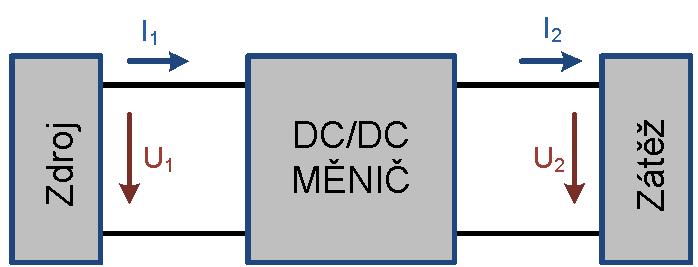
\includegraphics[width=0.7\linewidth]{patocka_pracovni_kvadranty_sch.pdf}
           \caption{Označení vstupních a výstupních veličin DC/DC měniče.}
           \label{enz:fig_prac_kvadranty_sch}
         \end{figure}

         Označme si vstupní a výstupní napětí a proud měniče podle obr.
         \ref{enz:fig_prac_kvadranty_sch}. Podle polarity výstupního napětí $U_2$ a výstupního
         proudu $I_2$ může měnič pracovat ve čtyřech kvadrantech tzv.\textbf{ VA-roviny} (viz obr.
         \ref{enz:fig_prac_kvadranty}).

         V kvadrantech \emph{1} i \emph{3} dodává měnič energii do zátěže. Je-li zátěží motor, tak
         pohání. Pasivní zátěže mohou pracovat pouze v těchto kvadrantech. V kvadrantech \emph{2} a
         \emph{4} dodává aktivní zátěž energii zpět do měniče. Jde-li o motor\footnote{Velikost
         napětí ss. motoru je úměrná otáčkám (rychlosti), polarita je dána směrem otáčení
         (uvažujeme motor s cizím buzením, např. s permanentními magnety). Velikost proudu je
         úměrná momentu na hřídeli, polarita je opět dána směrem momentu, tj. zda motor brzdí či
         pohání. Je třeba si povšimnout, že přechod mezi generátorickým a motorickým režimem mezi
         kvadranty 2 a 1 nebo mezi 3 a 4 (tj. takový, kdy se nemění polarita napětí, ale jen
         proudu) vůbec nemusí být na hřídeli motoru opticky pozorovatelný, neboť v dané chvíli
         přechodu se změní jen znaménko momentu (proudu) a přesto otáčky hřídele mohou být
         konstantní.}, pak brzdí.

      \subsubsection{Možnosti zapojení silového obvodu}\label{enz_kap_moznosti_zapojeni}
         \begin{figure}
           \centering
           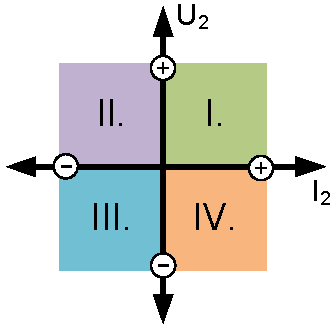
\includegraphics[width=0.5\linewidth]{patocka_pracovni_kvadranty.pdf}
           \caption{Pracovní kvadranty ve VA rovině.}
           \label{enz:fig_prac_kvadranty}
         \end{figure}
         Na první pohled jsou zřejmá určitá omezení:
         \begin{itemize}
       	   \item Indukčnost nikdy nesmí být zapojena paralelně ke vstupu či výstupu (protože tam je
                 napětí s nenulovou střední hodnotou).
           \item Kapacita nikdy nesmí být zapojena do série se vstupní nebo výstupní svorkou měniče
                 (protože tudy prochází proud s nenulovou střední hodnotou).
           \item Jako akumulační prvek nelze použít samostatně kapacitu, není-li v obvodu použita
                 ještě indukčnost (protože by v měniči napěťového typu docházelo k nepřípustnému
                 nárazovému nabíjení kondenzátoru zkratovým proudem). Čili měnič napěťového typu
                 musí obsahovat alespoň jednu indukčnost.
           \item Žádný spínač nesmí zkratovat vstup ani výstup měniče.
         \end{itemize}
      \subsubsection{Nejjednodušší měniče s jediným akumulačním 
                     prvkem}\label{ENZ:tit_menice_s_1_aku_prvkem} 
         Pro výchozí představu, vysvětlující princip činnosti, vytvoříme silový obvod měniče ze
         dvou prvků. Bude to indukčnost  \emph{L} a ideální přepínač. Vezmeme-li v úvahu omezení z
         kap. \ref{enz_kap_moznosti_zapojeni}, existují podle obr. \ref{enz:fig_DCDC_princip} jen
         tři způsoby, jak takový měnič zapojit \cite{Patocka}.

        \begin{figure}[ht!]
          \centering
          \begin{tabular}{c}
            \subfloat[$U_x=U_1\frac{t_1}{t_1+t_2}<U_1$]{\label{enz:fig_stepdown}
              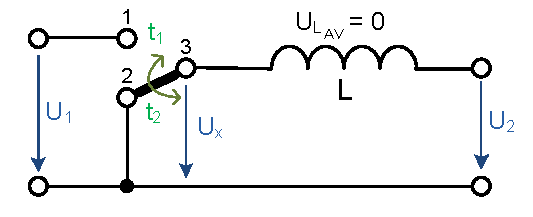
\includegraphics[width=0.8\linewidth]{patocka_step_down_princip.pdf}}     \\
            \subfloat[$U_x=U_2\frac{t_1}{t_1+t_2}>U_1$]{\label{enz:fig_stepup}
              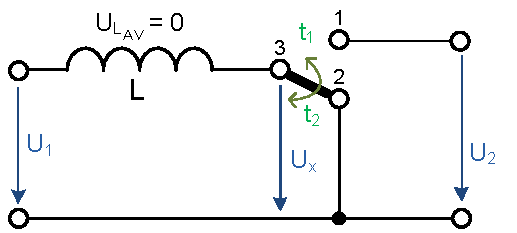
\includegraphics[width=0.8\linewidth]{patocka_step_up_princip.pdf}}       \\
            \subfloat[$U_x=\frac{U_1\cdot t_1 + U_2\cdot
                      t_2}{t_1+t_2}<>-U_1$]{\label{enz:fig_buckboost}
              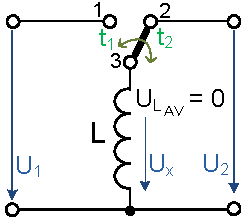
\includegraphics[width=0.7\linewidth]{patocka_buck_boost_princip.pdf}}
          \end{tabular}  
          \caption{Principiální schémata DC/DC měničů s jediným akumulačním prvkem.}
          \label{enz:fig_DCDC_princip}
        \end{figure}

        Označme střední hodnotu napětí mezi společným uzlem přepínače \texttt{3} a zemí jako 
        $U_x$. Předpokládejme, že přepínač je ovládán periodickým signálem s periodou $T$ a s
        nastavitelnou střídou, takže po dobu  $t_1$ spojuje svorky \texttt{3 - 1} a po dobu  $t_2 =
        T – t_1$ pak svorky \texttt{3 - 2}. Popišme nyní nejzákladnější vlastnosti tří měničů z
        obr. \ref{enz:fig_DCDC_princip}.

        \begin{enumerate}
          \item Střední hodnota $U_x$ na obr.\ref{enz:fig_stepdown} musí vzhledem k činnosti
                přepínače být:
                \begin{equation}\label{enz:stepdown_Ux}
                  U_x = U_1\frac{t_1}{t_1 + t_2} < U_1
                \end{equation}
                Výstupní napětí je rovno $U_x$, neboť střední hodnota napětí na indukčnosti L musí
                být nulová. Platí proto:
                \begin{equation}\label{enz:stepdown_U2}
                  U_2 = U_x = U_1\frac{t_1}{t_1 + t_2} < U_1
                \end{equation}
                Výstupní napětí je vždy menší než vstupní a má stejnou polaritu. Jde tedy o měnič
                \emph{snižující} a \emph{neinvertující}. Jeho jiné názvy jsou: \textbf{step-down,
                chopper, buck, propustný měnič}. Možné pracovní kvadranty jsou 1 a 2. Čili měnič je
                schopen dávat napětí $U_2$ jediné polarity, ale proud $I_2$ muže téci oběma směry
                (je-li to umožněno - aktivní zátěž).
          \item Střední hodnota $U_x$ na obr.\ref{enz:fig_stepup} musí vzhledem k činnosti
                přepínače být:               
                \begin{equation}\label{enz:stepup_Ux} 
                  U_x = U_2\frac{t_1}{t_1 + t_2} > U_1
                \end{equation}
                Vstupní napětí $U_1$ je rovno $U_x$ (nulová střední hodnota napětí na indukčnosti
                L). Odsud pro $U_2$ platí:
                \begin{equation}\label{enz:stepup_U2}
                  U_2 = U_1\frac{t_1 + t_2}{t_1} > U_1
                \end{equation}
                Střední hodnota výstupního napětí je vyšší než vstupní napětí a má stejnou polaritu.
                Jde tedy o \emph{zvyšující} a \emph{neinvertující} měnič. Jiný název je měnič
                \textbf{step-up, boost}. Možné pracovní kvadranty\footnote{Měnič
                \ref{enz:fig_stepdown} pracující v kvadrantu 1 je měničem \ref{enz:fig_stepup}
                pracujícím v kvadrantu 2. Naopak \ref{enz:fig_stepdown} v kvadrantu 2 je
                \ref{enz:fig_stepup} v kvadrantu 1. Čili \ref{enz:fig_stepdown} a
                \ref{enz:fig_stepup} je vlastně týž obvod, pouze zaměňuje vstup a výstup.} jsou opět
                1 a 2.
          \item Střední hodnota $U_x$ na obr.\ref{enz:fig_buckboost} musí vzhledem k činnosti
                přepínače být:
                \begin{equation}\label{enz:buckboost_Ux}
                  U_x = \frac{U_1t_1 + U_2t_2}{t_1 + t_2} <> - U_1
                \end{equation}
                Protože $U_x$ je střední hodnota napětí na indukčnosti L, musí platit $U_x =0$ tj.
                \begin{equation}\label{enz:buckboost_U2}
                  U_1 = - \frac{t_1}{t_2}U_1 <> - U_1
                \end{equation}
                Výstupní napětí má opačnou polaritu než vstupní, jde tedy o měnič
                \emph{invertující}. Velikost výstupního napětí může být větší i menší než vstupní.
                Vžité názvy jsou měnič \textbf{buck-boost, měnič se společnou tlumivkou, blokující
                měnič}. Možné pracovní kvadranty jsou 3 a 4.
        \end{enumerate}

      \subsubsection{Prakticky realizované silové obvody}\label{ENZ:subkap_silove_obvody}
        Kap. \ref{ENZ:tit_menice_s_1_aku_prvkem} ukazuje, že elektronicky ovládaný přepínač tvoří
        základní stavební kámen každého měniče. Tyto přepínače se ve skutečných obvodech realizují
        pomocí tzv. horních a dolních spínačů, což jsou \emph{trojpóly} podle obr.
        \ref{enz:fig_silove_obvody}.
        \begin{figure}
          \centering
          \begin{tabular}{c}
            \subfloat[Horní spínač]{\label{enz:fig_HS}
              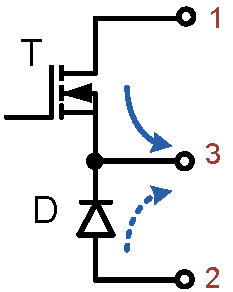
\includegraphics[width=0.3\linewidth]{patocka_horni_spinac.pdf}}     \\
            \subfloat[dolní spínač]{\label{enz:fig_LS}
              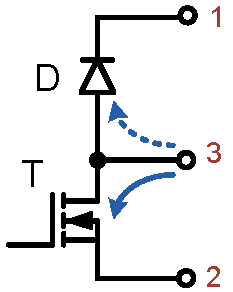
\includegraphics[width=0.3\linewidth]{patocka_dolni_spinac.pdf}}     \\ 
            \subfloat[Větev - paralelní kombinace horního a dolního spínače]{\label{enz:fig_arm}
              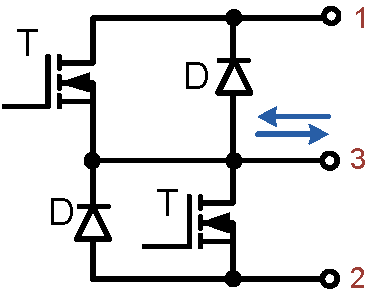
\includegraphics[width=0.4\linewidth]{patocka_vetev.pdf}}
          \end{tabular}  
          \caption{Horní a dolní spínač.}
          \label{enz:fig_silove_obvody}
        \end{figure}

        \begin{figure*}
          \centering
          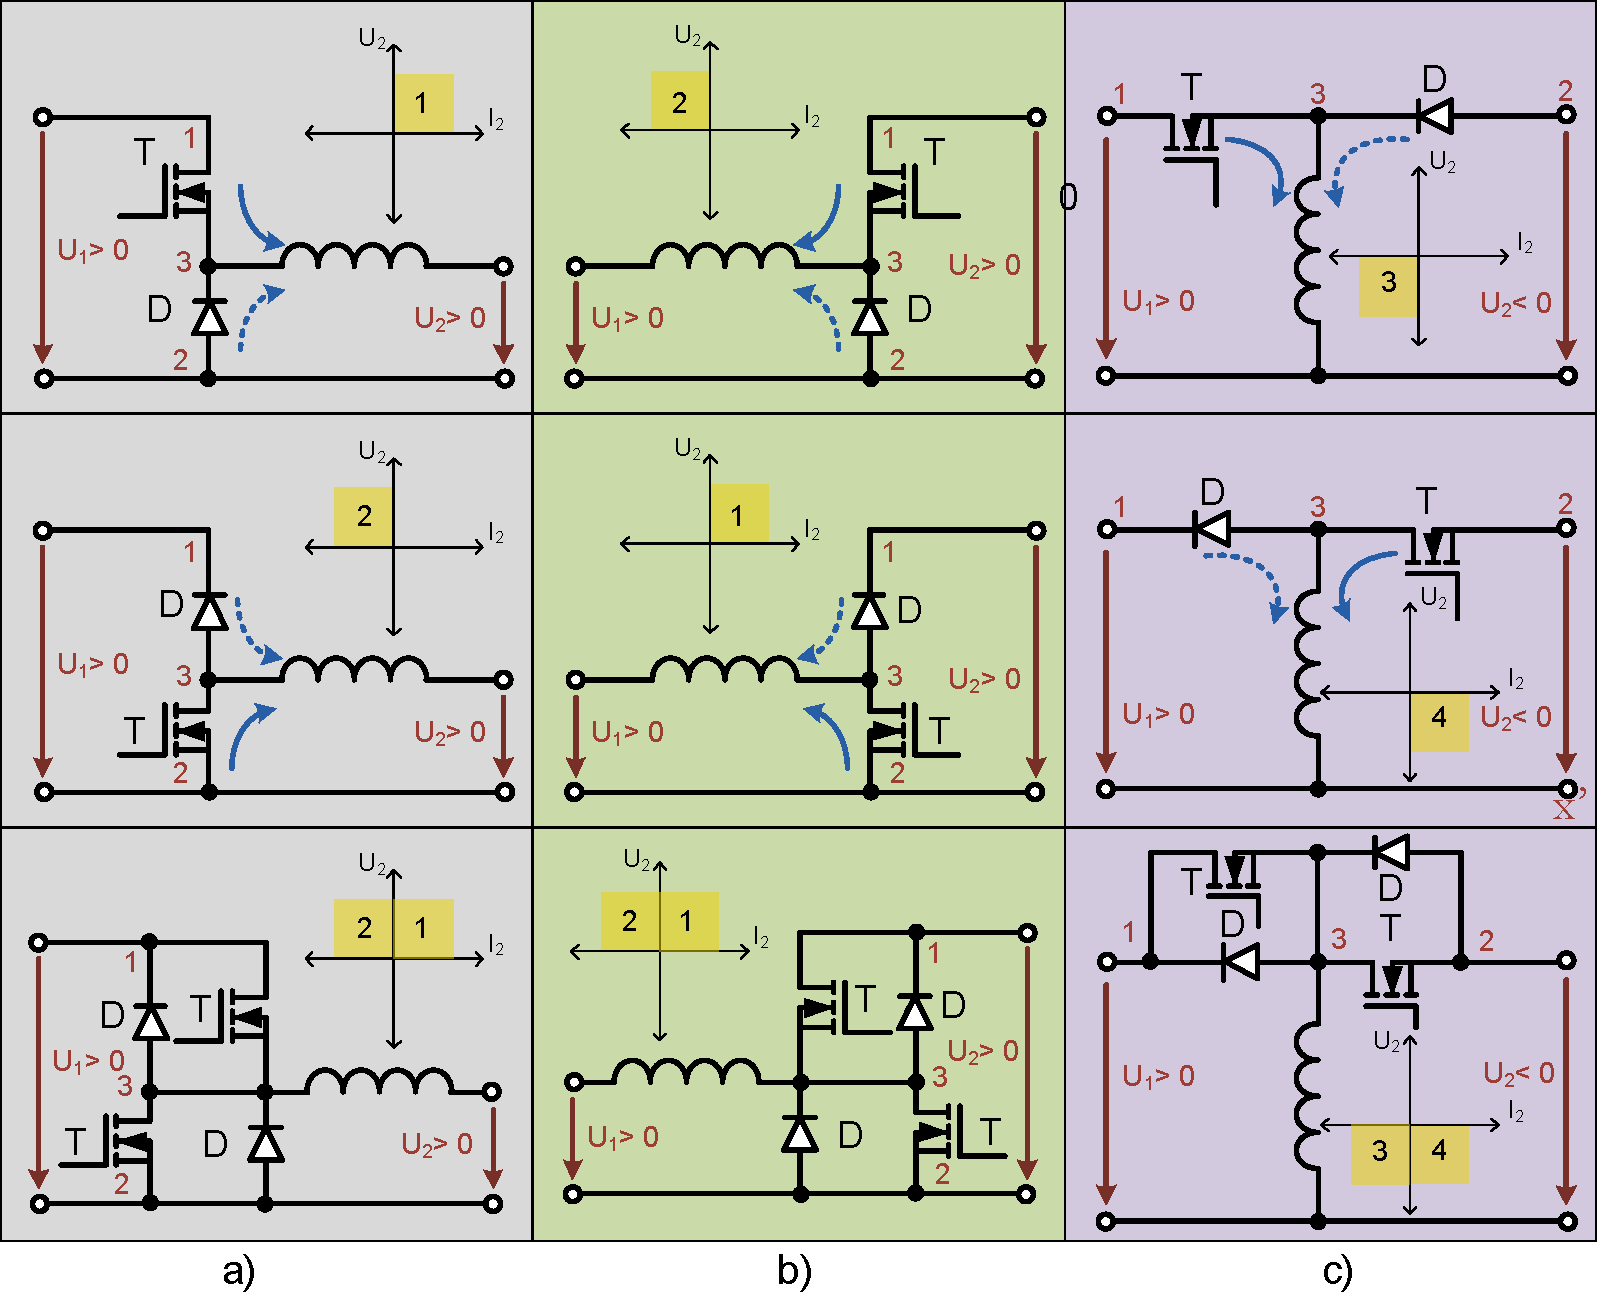
\includegraphics[width=0.9\textwidth]{patocka_silove_obvody_kvadranty.pdf}
          \caption[Skutečné silové obvody měničů a jejich kvadranty]{Skutečné silové obvody měničů
                   z obr. \ref{enz:fig_DCDC_princip} a jejich pracovní kvadranty: a) měnič snižující
                   neinvertující (step-down), b) měnič zvyšující neinvertující (step-up), c) měnič
                   invertující (buck-boost)}
          \label{enz:fig_silove_obv_kvadranty}
        \end{figure*}
        
\subsection{Step-down converter \newline(snižující neinvertující měnič)}\label{ENZ:kap_step_down}
  Jedná se o měnič s horním spínačem. Další jeho používané názvy jsou: propustný měnič, chopper,
  buck. \emph{Pracuje v 1. kvadrantu}.
  \begin{figure}[ht!]
    \centering
    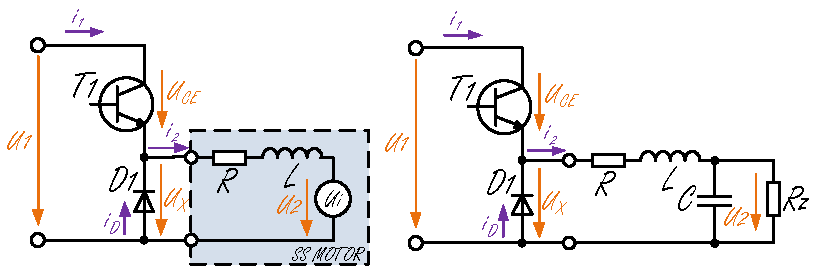
\includegraphics[width=1\linewidth]{patocka_step_down_sch1.pdf}
    \caption[Snižující měnič]{Snižující měnič pracující v prvním kvadrantu s aktivní zátěží
             typu stejnosměrný motor nebo s LC filtrem}
    \label{enz:fig_StepDown_sch1}
  \end{figure}

  \begin{figure}[ht!]
    \centering
    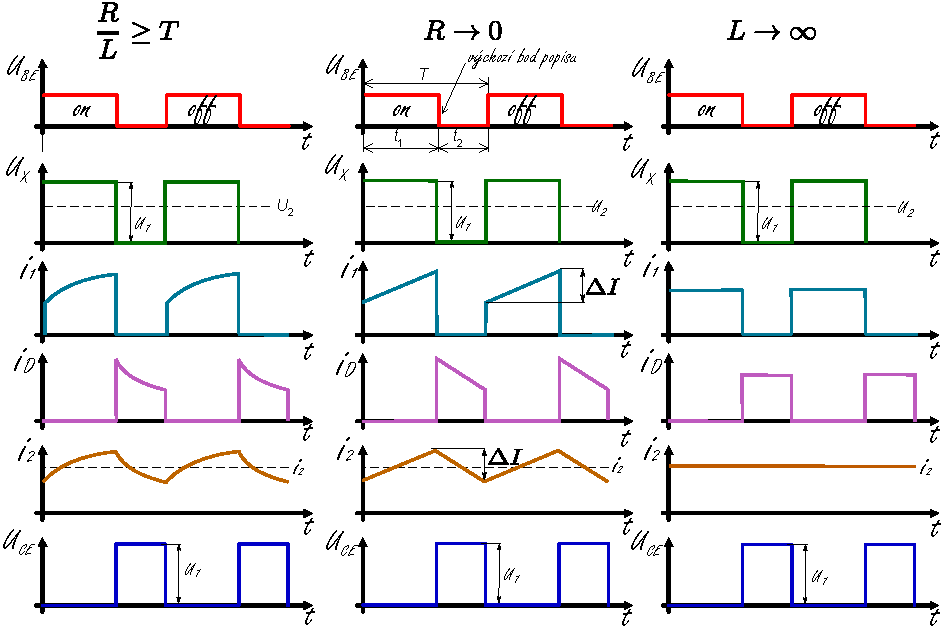
\includegraphics[width=1\linewidth]{patocka_step_down_waveform.pdf}
    \caption[Snižující měnič - průběhy]{Průběhy napětí a proudů snižujícího měniče}
    \label{enz:fig_StepDown_wave1}
  \end{figure}

\subsection{Step-up converter (zvyšující neinvertující měnič)}\label{ENZ:kap_step_up}
  \begin{figure}[ht!]
    \centering
    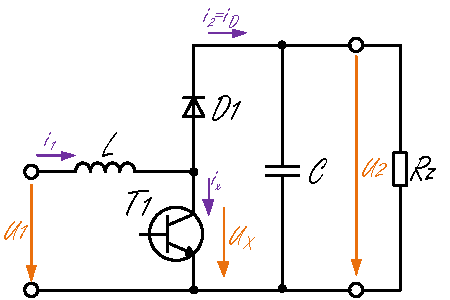
\includegraphics[width=0.8\linewidth]{patocka_step_up_sch1.pdf}
    \caption[Zvyšující měnič]{Zvyšujícího měnič pracující v prvním kvadrantu - Schéma zapojení}
    \label{enz:fig_StepUp_sch1}
  \end{figure}

\subsection{Buck-boost converter \newline(Invertující měnič se společnou tlumivkou)}\label{ENZ:kap_buck_boost}
\subsection{Cuk converter \newline(Měnič se společným konden\-zá\-to\-rem)}\label{ENZ:kap_cuk}
\subsection{SEPIC converter \newline(Single-ended primary inductor converter)}\label{ENZ:kap_sepic}         